\chapter{I farmaci}

Al fine di garantire un'ottima riuscita della procedura ed evitare nel bambino il ricordo di un'esperienza spiacevole e talora traumatica, ad oggi si può ricorrere sia ad interventi farmacologici di analgosedazione che ad interventi non farmacologici. Quest'ultimi possono essere utilizzati come metodo complementare o esclusivo, con innumerevoli benefici: dal ridurre l'agitazione preprocedurale e permettere una miglior transizione alla fase di sedazione, al contenere le dosi di farmaco utilizzate nel corso della procedura finanche, in alcuni casi, al prevenire del tutto il ricorso alla sedazione \cite{Uptodate}. Si tratta di approcci cognitivi e comportamentali che racchiudono tecniche di distrazione, rilassamento, desensibilizzazione e rinforzo positivo; risulta inoltre fondamentale, al fine di abbassare i livelli di ansia, instaurare una relazione di fiducia con i genitori e il bambino e definire un'adeguata strategia comunicativa, che adotti un linguaggio adeguato all'età o eventualmente introduca il gioco come strumento per prendere confidenza con le attrezzature mediche e le varie fasi della procedura. Tuttavia la sedazione farmacologica rimane la principale risorsa per agevolare le procedure più invasive. 

La scelta dell'agente farmacologico incide fortemente sulla qualità del risveglio post procedurale e va basata su diversi fattori. Premesso che il farmaco o la combinazione di farmaci selezionati deve indurre sedazione e analgesia adeguate a consentire il completamento della procedura con successo, mantenendo i riflessi protettivi delle vie aeree e l'autonomia cardiorespiratoria \cite{Krauss2006}, nel processo di decisione è importante valutare anche il livello di profondità della sedazione desiderato, conseguenza a sua volta del grado di analgesia richiesto dalla procedura. Infatti, talvolta è sufficiente solamente l'ansiolisi, altre volte è necessaria una più estesa analgesia, in altre occasioni invece lo scopo è quello di mantenere il paziente immobile, senza quindi bisogno di trattare il dolore. Altri elementi che guidano nella scelta del farmaco sono la familiarità nell'utilizzo da parte del sedatore e le caratteristiche individuali del paziente (età, comorbidità, allergie, grado di collaborazione, {\color{orange} ore di digiuno (?)}), che possono controindicare alcuni agenti farmacologici \cite{Uptodate}.
Infine, sono rilevanti alcune caratteristiche farmacocinetiche: sono infatti preferenziali farmaci con molteplici vie di somministrazione, induzione rapida e breve emivita, tale da concedere un celere recupero con assenti o minimi effetti collaterali.

Di seguito verranno dunque analizzate e confrontate le proprietà, i dosaggi, le indicazioni e gli effetti collaterali dei farmaci più comunemente utilizzati al di fuori della sala operatoria. 

\section{Propofol}

Il propofol è un sedativo ipnotico, non analgesico, il cui meccanismo d'azione a livello del sistema nervoso centrale non è del tutto noto, anche se ne è stata studiata l'interazione con il recettore A dell'acido $\gamma$-amminobutirrico (GABA) \cite{Propofol2015}.

\subsection*{Farmacodinamica}

Il legame tra le molecole di propofol e il recettore ionotropico GABA-A è responsabile degli effetti centrali del farmaco. Questo recettore è costituito da un complesso proteico associato ad un canale per il cloro ed è presente a livello postsinaptico di molti neuroni. Una volta riconosciuto il ligando, si verifica un aumento del flusso degli ioni cloro attraverso la membrana, determinando iperpolarizzazione del neurone ed un conseguente effetto inibitorio, con minor eccitabilità e risposta agli stimoli esterni \cite{Propofol2015}.

\subsection*{Farmacocinetica}

Uno dei motivi per cui il propofol è ampiamente utilizzato riguarda proprio le sue vantaggiose caratteristiche farmacocinetiche: ha infatti un esordio d'azione estremamente rapido (30-45 secondi) ed un altrettanto rapido risveglio (5-15 minuti dopo singolo bolo, più lento in caso di infusione continua o boli multipli) \cite{Simeupsedazione, Uptodatepharmacology}. Si tratta di una molecola liposolubile, che supera la barriera ematoencefalica, macroscopicamente il propofol assume un aspetto lattescente e può essere somministrato solo per via endovenosa. Nel momento dell'iniezione può causare bruciore locale, che può essere prevenuto utilizzando una vena di calibro maggiore o diluendo a metà il propofol con soluzione fisiologica (5 mg/mL) \cite{Simeupsedazione}. 

\subsection*{Posologia}

Viene somministrato con un dosaggio di 1-2 mg/kg come bolo iniziale d'induzione, seguito da successivi boli multipli da 0.5 a 1 mg/kg ogni 2-3 minuti. Per le procedure più lunghe può anche essere utilizzato in infusione continua.
La dose massima è di 10 mg/kg totali per procedura \cite{Simeupsedazione}.

\subsection*{L'associazione con la ketamina}

Se la procedura è dolorosa il propofol può essere dato in combinazione con la ketamina, che oltre ad avere un'importante azione analgesica controbilancia gli effetti ipotensivo e bradicardizzante del propofol. Esistono in commercio delle formulazioni chiamate \emph{ketofol} con diversi rapporti di ketamina e propofol, tra i vantaggi risalta anche una minor incidenza di vomito e agitazione al risveglio, poiché l'effetto combinato permette di risparmiare ketamina \cite{Simeupsedazione}.

\subsection*{Effetti collaterali}

I principali effetti collaterali del propofol sono rappresentati dalla depressione respiratoria e dalla conseguente apnea, che dipendono dal dosaggio, dalla velocità di somministrazione e dalla risposta soggettiva del paziente. Inoltre, il propofol può determinare ipotensione e più raramente bradicardia \cite{propofolsafety2010}.
Un altro temibile quanto raro effetto avverso è costituito dalla \emph{sindrome da infusione di propofol}, potenzialmente fatale e descritta sia negli adulti che nei bambini \cite{Propofolinfusionsyndrome2019}. Si tratta di un insieme di segni e sintomi che si verifica in pazienti critici, che ricevono propofol in infusione a dosaggi elevati (>5 mg/kg/h) o per un periodo prolungato (>48h) ed è caratterizzata dalla presenza di una o più delle seguenti alterazioni, non spiegabili altrimenti: acidosi metabolica, rabdomiolisi, variazioni elettrocardiografiche associate o meno ad AKI, iperkaliemia, dislipidemia, scompenso cardiaco, febbre, elevazione degli enzimi epatici o del lattato. 

\section{Ketamina}

La ketamina è un farmaco anestetico dissociativo derivato dalla fenilciclidina con potenti proprietà sedative, analgesiche ed amnesiche. E' stato introdotto in commercio per la prima volta nel 1970 e da allora viene largamente utilizzato per lo più in ambito anestesiologico ma possiede un'ampia gamma di possibili applicazioni cliniche \cite{Ketamineapplication2019}: dal trattamento del dolore cronico, anche in pazienti oncologici, al trattamento del disturbo depressivo maggiore, grazie ai suoi effetti antidepressivo ed antisuicidario. Inoltre, mentre rimane controverso il suo ruolo nel trattamento dell'asma, sono riconosciute le sue azioni antinfiammatoria ed immunomodulatrice, a cui si aggiungono quella antiproliferativa ed apoptotica, che vengono studiate con interesse per la ricerca sulla soppressione tumorale.

\subsection*{Farmacodinamica}

La ketamina è un farmaco che porta il paziente in uno stato dissociativo, simile alla trance, in cui l'individuo rimane parzialmente vigile ma con una depressione della consapevolezza: mantiene infatti gli occhi aperti ma non interagisce con l'ambiente circostante e non percepisce dolore. A differenza di altri farmaci non presenta un \emph{continuum della sedazione}, piuttosto l'effetto è presente o assente a seconda del dosaggio. Viene scelta per la sua ottima capacità analgesica e l'alto profilo di sicurezza, in quanto permette il mantenimento dei riflessi protettivi delle vie aeree e non deprime il centro del respiro; inoltre dal punto di vista cardiovascolare aumenta la frequenza cardiaca e la pressione arteriosa \cite{Krauss2006}. 
\\La ketamina esercita le sue proprietà attraverso l'interazione con diversi recettori. Tuttavia, la maggior parte degli effetti sono dovuti al blocco dei recettori NMDA (\emph{N-Metil-D-Aspartato}, ai quali il farmaco si lega come antagonista non competitivo. Si tratta di canali ionici glutammatergici permeabili agli ioni calcio, i quali normalmente sono implicati nell'attivazione di diversi pathway intracellulari \cite{Zanos2018}.
\\La ketamina esiste sotto forma di due enantiomeri \footnote{Sono isomeri ottici, ovvero entità molecolari speculari e non sovrapponibili.} :levogiro (S) e destrogiro (R). La forma levogira ha un maggior attività anestetica ed analgesica, favorisce una miglior immobilità del paziente e un recupero più rapido, mentre la forma destrogira è più efficace per l'uso antidepressivo \cite{Simeupsedazione}.

\subsection*{Farmacocinetica}

La ketamina è altamente liposolubile, si distribuisce ai tessuti periferici e supera rapidamente la barriera ematoencefalica. Viene preferenzialmente somministrata per via endovenosa o intramuscolare ma, seppur con una biodisponibilità inferiore, può essere utilizzata anche attraverso altre vie: intranasale, rettale ed orale. \cite{Simeupsedazione, Ketamineapplication2019}. 
\\La ketamina viene metabolizzata per l'80\% dal fegato in norketamina, che mantiene un terzo delle proprietà della molecola originale e viene eliminata per via urinaria. 
\\Per via endovenosa ha un inizio d'azione molto rapido, che avviene entro 1-2 minuti dalla somministrazione, anche la durata è breve (10-15 minuti) con un tempo di risveglio di circa 30-60 minuti \cite{Uptodatepharmacology}. Mentre la somministrazione per via intramuscolare ha un inizio d'azione di 10-15 minuti e una durata della sedazione di 30-40 minuti \cite{Berkenbosch2015}.

\subsection*{Indicazioni}

Questo farmaco viene comunemente utilizzato sia in urgenza che in elezione. Viene scelto principalmente per procedure dolorose e di breve durata, quali la riduzione di una frattura o la sutura di una ferita. Può essere usato anche in combinazione con il propofol, al fine di aumentare il grado di sedazione e migliorare il profilo emodinamico, durante procedure d'elezione, quali colonscopie o aspirati midollari. Inoltre, per le sue caratteristiche neuroprotettive, viene spesso scelta in caso di intubazione d'urgenza di pazienti con traumi cranici severi \cite{Simeupsedazione}.

\subsection*{Posologia}

Una caratteristica distintiva della ketamina consiste nell'avere una relazione diretta tra la dose e l'effetto che si vuole ottenere, non esiste infatti per questo farmaco un \emph{continuum} tra i diversi livelli di sedazione. Vengono riportati nella seguente tabella \ref{tab:1} i dosaggi per via endovenosa associati all'intento terapeutico che si vuole raggiungere.


\begin{table}[!h]
    \centering
    \begin{tabular}{|l|l|}
       Scopo terapeutico     & Dosaggio \\ \hline
       Analgesia & 0.1-0.3 mg/kg  \\
       Aspetto ricreazionale & 0.3-0.6 mg/kg \\
       Sub-dissociativa & 0.4-0.8 mg/kg \\
       Analgosedazione & 0.8-1 mg/kg 
    \end{tabular}
    \caption{Adattata dal Manuale Simeup per la sedazione procedurale in pediatria \cite{Simeupsedazione}}
    \label{tab:1}
\end{table}

\bigskip

La posologia relativa alle altre vie di somministrazione è, invece la seguente: 
\begin{itemize}
    \item via intramuscolo: 4-5 mg/kg
    \item via intranasale: 1-3 mg/kg (max. 1 mL per narice)
    \item via orale: 5-10 mg/kg
\end{itemize}

\subsection*{Effetti collaterali}

Il principale svantaggio di questo agente farmacologico è rappresentato dalla lunga lista di effetti avversi che possiede. Il più temibile è rappresentato dal laringospasmo, che si può verificare soprattutto in seguito a stimolazione delle prime vie aeree, conseguente ad esempio a scialorrea, altro effetto collaterale della ketamina, oppure a gastroscopia. Inoltre, l'utilizzo di alte dosi di ketamina può causare allucinazioni e deliri al risveglio, il cosiddetto \emph{bad trip}. Si tratta di episodi solitamente autorisolventi in poche ore ma spiacevoli per il paziente e i genitori; i casi più intensi possono beneficiare della somministrazione di benzodiazepine \cite{Simeupsedazione}. Altri effetti collaterali minori ma frequenti (8\%) sono rappresentati dalla nausea e dal vomito, che possono essere prevenuti tramite la somministrazione di ondansetron (0.15 mg/kg), un antiemetico \cite{Uptodatepharmacology}. Inoltre, la ketamina può determinare la comparsa di nistagmo orizzontale, un effetto privo di significato clinico \cite{Simeupsedazione}. 
\\L'insorgenza di reazioni avverse è più frequente se il farmaco è stato somministrato a dosaggi superiori o inferiori a quelli terapeutici, mentre la combinazione con il propofol porta ad una minor incidenza di agitazione al risveglio e vomito, poiché permette di ridurre le dosi di ketamina utilizzata durante la procedura \cite{Simeupsedazione, Shah2011}. 

\subsection*{Controindicazioni}

L'uso della ketamina è controindicato in termini assoluti nei lattanti con meno di tre mesi di vita, che risultano, anche per motivi anatomici, più soggetti a reazioni respiratorie gravi \cite{Zanos2018}; negli affetti da schizofrenia, in quanto gli effetti psicoattivi della ketamina possono esacerbare i sintomi; infine nei pazienti che hanno avuto precedentemente gravi reazioni collaterali \cite{Uptodatepharmacology}.
\\Altre controindicazioni relative, invece, riguardano soggetti con: instabilità delle vie aeree, infezioni o patologie polmonari attive, patologie cardiovascolari tra cui ipertensione, angina o scompenso cardiaco, porfiria, tireopatie e assunzione di farmaci per la tiroide, che possono aumentare l'effetto simpaticomimetico. Inoltre, un età compresa tra 3 e 12 mesi, un aumentata pressione intracranica dovuta a lesioni occupanti spazio e un aumentata pressione intraoculare, conseguente a glaucoma od altre lesioni oculari sono controindicazioni attualmente messe in dubbio e non più suffragate \cite{Green2011, Simeupsedazione}.   

\section{Midazolam}

Il midazolam è una benzodiazepina a breve durata d'azione, che possiede proprietà ansiolitiche, sedative, amnesiche, anticonvulsivanti, ipnoinducenti e miorilassanti; non possiede tuttavia azione analgesica \cite{Krauss2006}. 
\\ \`E il farmaco più comunemente usato per la sedazione minima (o ansiolisi) in ambito pediatrico, inoltre può essere utilizzato con un adeguato profilo di sicurezza fino a un livello di sedazione moderato \cite{Manso2019}. Per una maggior profondità, invece, è preferibile l'associazione con altri agenti farmacologici, al fine di prevenirne gli effetti avversi dose-correlati.

\subsection{Farmacodinamica}

Il meccanismo d'azione delle benzodiazepine è dovuto al potenziamento dell'attività inibitoria neuronale, fisiologicamente esercitata dal legame tra il neurotrasmettitore GABA e i suoi recettori. Esistono due tipi di recettori per l'acido $\gamma$-amminobutirrico: i recettori ionotropici GABA-A e i recettori metabotropici GABA-B. Le benzodiazepine si legano alla subunità $\gamma$ dei recettori GABA-A in modo esclusivo e con una maggior affinità rispetto al neurotrasmettitore endogeno, che invece si lega alla subunità $\beta$ degli stessi. Ne consegue un maggior effetto di depressione neuronale, grazie allo stesso meccanismo descritto poco sopra nella sezione di farmacodinamica del propofol \cite{Olkkola2008}. 
\\Come schematicamente rappresentato nella figura \ref{fig:benzo}, gli effetti clinici si susseguono dall'ansiolisi alla sedazione fino all'ipnosi in relazione al grado di saturazione dei recettori GABA-A, che dipende a sua volta dalla concentrazione ematica del farmaco. 

\begin{figure}[!h]
    \centering
    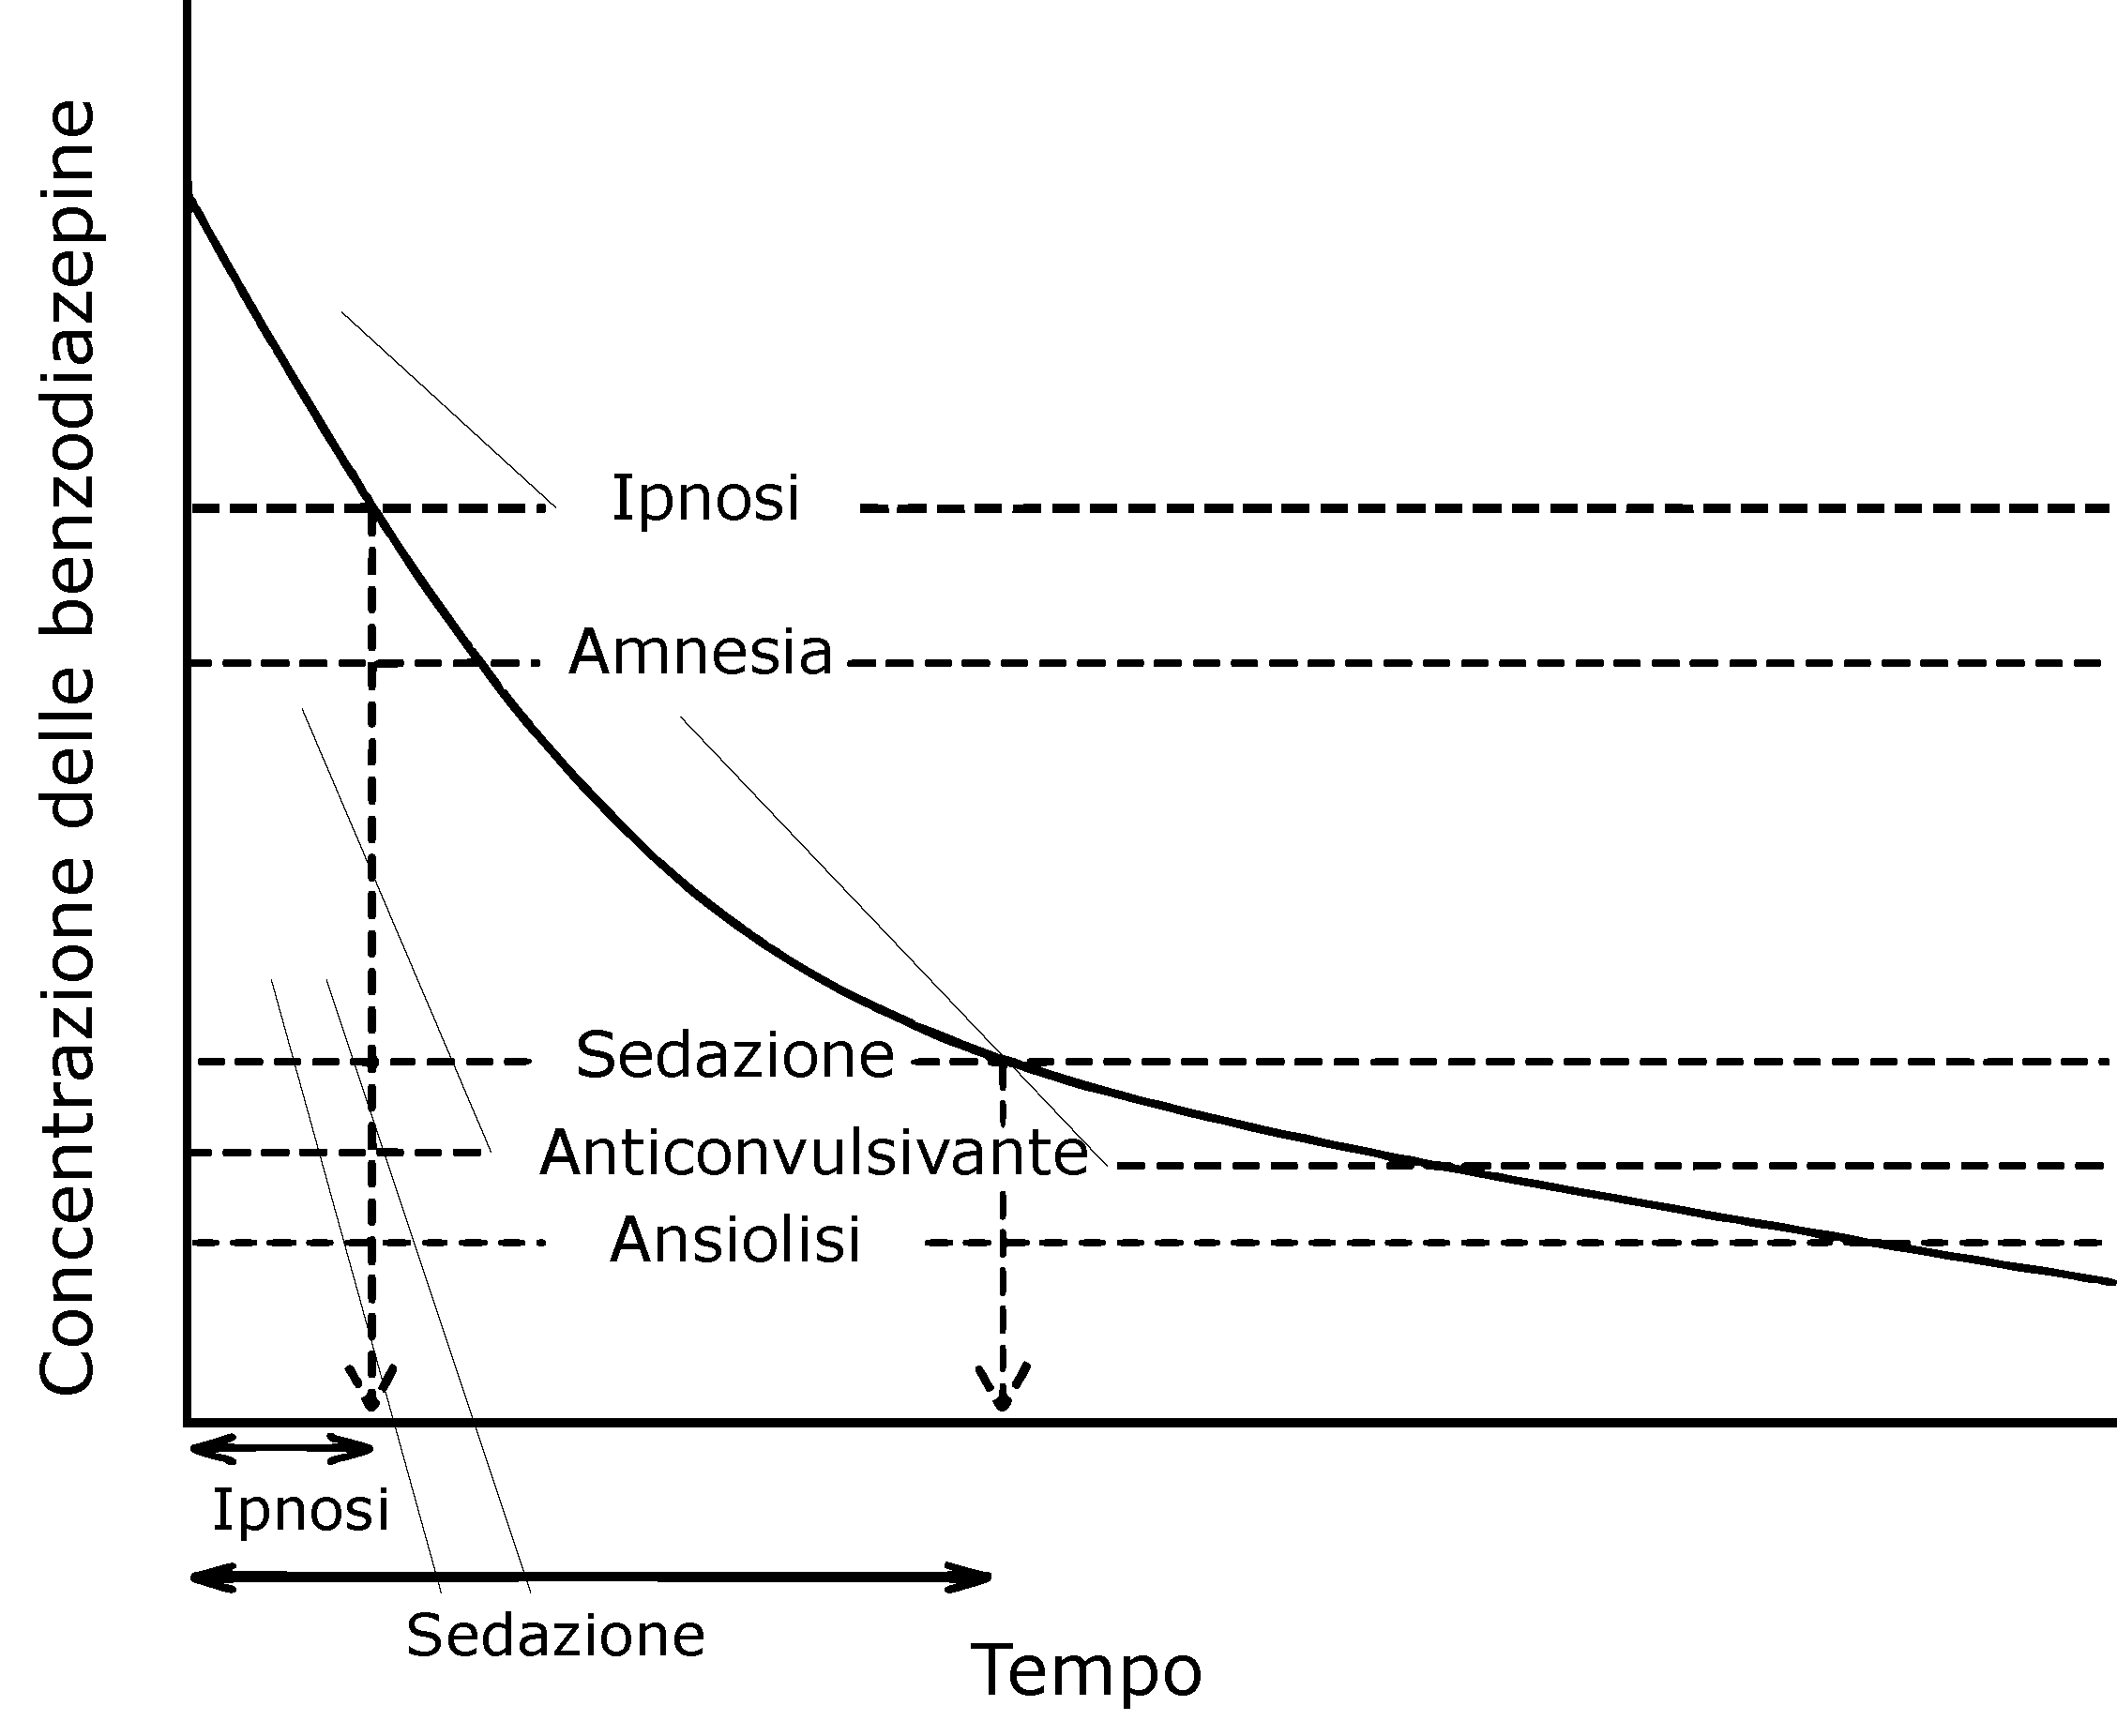
\includegraphics[width=0.7\textwidth]{Figure/figurabenzo.pdf}
    \caption{Relazione tra la concentrazione ematica delle benzodiazepine e i diversi effetti clinici ottenibili, immagine adattata da \cite{Olkkola2008}.}
    \label{fig:benzo}
\end{figure}

\subsection{Farmacocinetica}

\section{Dexmedetomidina}

\lipsum[4]

\section{Protossido di azoto}

\lipsum[5]
 